\documentclass[../uilmath.tex]{subfiles}
\graphicspath{{\subfix{../figures/}}}
\begin{document}
\chapter{Extra Topics}
\section*{Problems}
\begin{enumerate}[label=\bfseries\arabic*.]
    \item %% Problem 1
    Which equality axiom of addition is demonstrated by $(ax+by)+c=ax+(by+c)$?

    \item %% Problem 2
    Which of the following numbers is considered to be an ``abundant'' number?

    $\textbf{(A) } 26 \qquad \textbf{(B) } 28 \qquad \textbf{(C) } 30 \qquad \textbf{(D) } 32 \qquad \textbf{(E) } 34$

    \item %% Problem 3
    $ABC1_{16}+ABC1_{15}=\blank_{14}$

    \item %% Problem 4
    Let $P={2,3,5}, Q={2,4,6}$, and $R={3,5,7}$. How many elements are in $(P\cap R)\cup(R\cap Q)$?

    \item %% Problem 5
    Which of the following sets is closed under addition and subtraction?

    $\textbf{(A) } \text{Positive Even Numbers} \qquad \textbf{(B) } \text{Integers} \qquad \textbf{(C) } \text{Positive Odd Numbers} \qquad \textbf{(D) } \text{Primes} \qquad \textbf{(E) } \text{Wholes}$

    \item %% Problem 6
    Find the harmonic mean of 4 and 9.

    \item %% Problem 7
    Which of the following numbers is considered to be an ``deficient'' number?

    $\textbf{(A) } 24 \qquad \textbf{(B) } 56 \qquad \textbf{(C) } 66 \qquad \textbf{(D) } 92 \qquad \textbf{(E) } 112$

    \item %% Problem 8
    In the decimal number $2x3y4z$, the letters $x$, $y$, and $z$ represent digits where all six digits are distinct.
    If the number is divisible by 30 then $x+y+z$ could be: 

    \item %% Problem 9
    $888_9 + 555_6 + 222_3 = \blank_3$

    \item %% Problem 10
    Use the Fibonacci characteristic sequence $\dots -1.5,p,q,3,r,\dots$ to Find $p+q+r$.

    \item %% Problem 11
    One of Eratosthenes of Cyrene's main contributions to mathematics involved a method for finding \blank .

    \item %% Problem 12
    I'm an unhappy deficient number but a number that is lucky to be prime. Which of the following numbers am I?

    \item %% Problem 13
    Which equality axiom of multiplication is demonstrated by $(a)(a)^{-1}=1$?

    \item %% Problem 14
    How many subsets containing 4 members can be made from the set ${2,1,3,4,7,11}$?

    \item %% Problem 15
    Which of the following was the first Nigerian woman to be awarded a doctorate in mathematics?

    \item %% Problem 16
    Find the harmonic mean of the roots of $x^3-7x^2+14x-8=0$.

    \item %% Problem 17
    If $R$, $S$, and $T$ are distinct digits then $RST_2-ST_3-R_4$ has a numeric value in base 10 of:

    \item %% Problem 18
    The set ${\dots, -6, -4,-2,0,2,4,6,\dots}$ is closed under which of the following operations:
    \begin{center}
        I. addition \qquad II. subtraction \qquad III. multiplication \qquad IV. division 
    \end{center}

    \item %% Problem 19
    $F_0=0$ and $F_1$ are the first two Fibonacci numbers. Find $F_{10}$.

    \item %% Problem 20
    Let $R={1,3,5}, S={0,2,4}$, and $T={1,2,3}$. How many elements are in $(R\cup T)\cap(S\cup T)$?

    \item %% Problem 21
    $(p-q)\times r = pr-qr$ is an example of which property of equality?

    \item %% Problem 22
    The 8th Fibonacci number is 13. The 10th Fibonacci number is 34. Find the 9th Lucas number.

    \item %% Problem 23
    Find $L_9$ if $L_0=2,L_1=1$, and $L_n=L_(n-1)+L_(n-2)$, where $n\geq 2$.

    \item %% Problem 24
    The universal set $U={2,3,5,7,11,13,15,17,19}$. Subset $L={5,7,15,17}$, subset $M={3,13}$. 
    How many elements are in the complement set of $L\cup M$?

    \item %% Problem 25
    Which of the following mathematicians was most remembered as the inventor of logarithms?

    \item %% Problem 26
    In the binomial expansion of $(3x-1)^5$, the coefficient of the fourth term is:

    \item %% Problem 27
    What are the odds that a factor of 2010 is a prime number?

    \item %% Problem 28
    The formula $e^{ix}=\cos x + i\sin x$, where $e$ is the base of the natural logarithm and $i$ is the imaginary unit, is named after:

    \item %% Problem 29
    The odd numbers from 1 to 17 are to be placed in this magic square in which the rows and columns have the same sum. Find the value of $x$.
    \begin{center}
        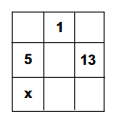
\includegraphics[width=0.3\textwidth]{2010A28.PNG}
    \end{center}

    \item %% Problem 30
    $P={p,l,u,s}, Q={m,i,n,u,s}$, and $R={t,i,m,e,s}$. How many elements are in $(P\cup Q)\cap (P\cup R)$?

    \item %% Problem 31
    The number 12010 in base 3 is equivalent to the number $wxyz$ in base 5, where $w$, $x$, $y$, and $z$ are digits. Find $w+x+y+z$.

    \item %% Problem 32
    $3(x+4)=5$ and $3(4+x)=5$ is an example of the \blank property.

    \item %% Problem 33
    If $ax+b=c$ and $c=dx+e$, then $ax+b=dx+e$ is an example of the \blank property.

    \item %% Problem 34
    Which of the following is true about the relation graphed below?
    \begin{center}
        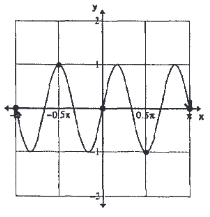
\includegraphics[width=0.3\textwidth]{2010B16.PNG}
    \end{center}

    \item %% Problem 35
    Integers $x$ \& $y$ exist such that $x=2y$ and the arithmetic mean of $x$ \& $y$ is 1 more than the harmonic mean of $x$ \& $y$. Find the geometric mean of $x$ \& $y$.

    \item %% Problem 36
    The figure shown is reflected over a negative diagonal. Which of the following figures is the result of that single transformation?
    \begin{center}
        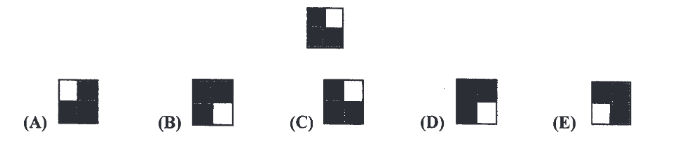
\includegraphics[width=0.7\textwidth]{2010B23.PNG}
    \end{center}

    \item %% Problem 37
    A recent visit to the planet Strangebase discovered that the equation, $3S^2-25S+66=0$, has two solutions, 4 and 9. What base was being used for the number system on planet Strangebase?

    \item %% Problem 38
    Evaluate: $\prod_{n=2}^6 (1+\frac{1}{n})$

    \item %% Problem 39
    Which of the following mathematicians created an abacus for calculating products and quotients and extracting square roots that was based on Arab mathematics and lattice multiplication.

    \item %% Problem 40
    Polly Euler folds the net shown into a cube. What letter will be on the opposite side of side $S$?
    \begin{center}
        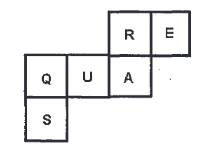
\includegraphics[width=0.3\textwidth]{2010B34.PNG}
    \end{center}

    \item %% Problem 41
    If $\sqrt{x\sqrt[3]{x\sqrt[4]{x}}}=\sqrt[n]{x^k}$, where $k$ and $n$ are relatively prime, then $k=$?

    \item %% Problem 42
    The universal set $U={1,2,3,5,8,13,21,34}$. Subset $A={1,3,8,21,34}$ and subset $B={2,3,5,13,21}$. How many elements are in the complement set of $A\cap B$?

    \item %% Problem 43
    Which of the following numbers is an unhappy number and evil number?

    $\textbf{(A) } 7 \qquad \textbf{(B) } 8 \qquad \textbf{(C) } 9 \qquad \textbf{(D) } 10 \qquad \textbf{(E) } 11$

    \item %% Problem 44
    $2\times 4\times 8 = 8\times 8 = 64$ and $2\times 4\times 8 = 2\times 32 = 64$ are examples of the ? property of equality.

    \item %% Problem 45
    If $2(3+5)=16$ and $16=4^2$ then $2(3+5)=4^2$. Which of the following properties does this example illustrate?

    \item %% Problem 46
    Pauline Gone folds the net shown into a cube. What letter will be on the opposite side of face $E$?
    \begin{center}
        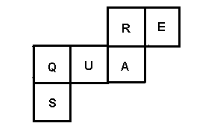
\includegraphics[width=0.3\textwidth]{2018A20.PNG}
    \end{center}

    \item %% Problem 47
    Find $a+b+c+d$ given the Fibonacci characteristic sequence: $3,a,b,17,c,d,71,\dots$.

    \item % Problem 48
    Which of the following mathematicians is known for developing a ``machine'' that uses a system of rules, states, and transitions 
    used to decide a language or to solve mathematical functions? It is a powerful tool used in computer science and code breaking?

    \item %% Problem 49
    Mr. White's `bath tub mat' pattern table consists of 19 columns and 12 rows. Only 7 rows are shown. Determine the sum of the numbers in the 8th row.
    \begin{center}
        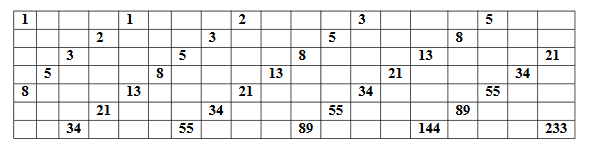
\includegraphics[width=0.3\textwidth]{2018A34.PNG}
    \end{center}

    \item %% Problem 50
    The harmonic mean of the real roots of $3x^3+2x^2+5x+4=0$ is \blank .

    \item %% 51
    Which of the following pairs of numbers are considered to be `fangs' of a `vampire' number?

    I. (35, 41) \qquad II. (21, 87) \qquad III. (72, 27) \qquad IV. (51, 63)

    \item %% 52
    Let $4022_b - k_b = 1665_b$, where $k_b$ is a four digit number. Find $k_b$ in base 10.

    \item %% 53
    7,158,AB3 $\div$ 9 has a remainder of 7. Find $A+B$.

    \item %% 54
    A square-free semiprime is a composite number that is the product of two different primes. How many composite numbers less than 20 are considered square-free semiprimes?

    \item % 55
    Let $U$ (universal set) $= {u,i,l,m,a,t,h,b}$, $B={b,u,i,l,t}$, and $T={t,h,u,m,b}$. Let $I=(B \cap T)^C$. Set $I$ contains how many distinct elements?

    \item %% 56
    Which of the following sets of numbers is closed under multiplication and addition?

    I. Primes \qquad II. Integers \qquad III. Wholes \qquad IV. Rationals 

    \item % 57
    For how many different positive integers $n$ is each of $n$, $n+2$, and $n+4$ a prime number?

    \item % 58
    What's the only positive integer whose two largest divisors have a sum of 111?

    \item % 59
    For how many different pairs of positive integers $(a,b)$, with greatest common factor 1, and with $a>b$, does $ab=30!$? (Note: $30!$ is the product of the first 30 positive integers.)

    \item % 60
    Leonardo Pisano Bigollo was an Italian mathematician who referenced and made known which of the following special sequences of numbers to Western mathematics?

    \item % 61
    Which of the following numbers is an abundant, happy, and lucky number?

    $\textbf{(A) } 28 \qquad \textbf{(B) } 31 \qquad \textbf{(C) } 44 \qquad \textbf{(D) }\text{all of these} \qquad \textbf{(E) } \text{none of these}$

    \item % 62
    Find $a+b+c+d$ given the Fibonacci characteristic sequence: $a,2,b,c,20,d,51,\dots$.

    \item % 63
    The set of Lucas numbers is ${1,3,5,7,11,\dots}$, where $L_1 = 1$. The set of Fibonacci numbers is ${1,1,2,3,5,\dots}$, where $F_1=1=F_2$.
    If $L_{10}=F_x+F_y$, where $y>x$, then $y$ is \blank .

    \item % 64
    If the following pattern continues, determine which of the following numbers will be in row 10.
    \begin{center}
        1 \qquad \text{row 0}\\
        1 \quad 1 \qquad \text{row 1}\\
        1 \quad 2 \quad 1 \qquad \text{row 2}\\
        1 \quad 3 \quad 3 \qquad \text{row 3}\\
        1 \quad 4 \quad 6 \quad 4 \quad 1 \qquad \text{row 4}\\
        1 \quad 5 \quad 10 \quad 10 \quad 5\quad 1 \qquad \text{row 5}
    \end{center}

    \item % 65
    An ``emirp'' number is a prime number that becomes a new prime number when the digits are reversed. Single digit primes and 
    palindromic primes cannot be emirp numbers. How many prime numbers less than 20 are considered to be emirp numbers?

    \item % 66
    Let $(131_b)\times 3_b = k_b$, where $k_b$ is a 3-digit number. Find $b$ if $k_b = 1323_4$.

    \item % 67
    If $P$, $Q$, and $R$ are different digits, then the largest possible three-digit sum for $PPP+QP+P=$? has which of the following forms?

    \item %68
    Let $A={a,c,u,t,e}, O={o,b,t,u,s,e}$, and $R={r,i,g,h,t}$. The number of elements in $(A\cup R)\cap O$ is:

    \item % 69
    $111A09201B\div 9$ has a remainder of 5. Find the least value of $A+B$.

    \item % 70
    Which of the following mathematicians is noted for his work with sets, probability, and logic?
    
    \item % 71
    

\end{enumerate}

\section*{Solutions}
\begin{enumerate}[label=\bfseries\arabic*.]
    \item %% Problem 1
    Associative 

    \item %% Problem 2
    C  

    \item %% Problem 3
    21411

    \item %% Problem 4
    2

    \item %% Problem 5
    B 

    \item %% Problem 6
    $5 \frac{7}{13}$

    \item %% Problem 7
    D 

    \item %% Problem 8
    12 

    \item %% Problem 9
    689

    \item %% Problem 10
    6.75

    \item %% Problem 11
    prime numbers 

    \item %% Problem 12
    37

    \item %% Problem 13
    Commutative

    \item %% Problem 14
    15

    \item %% Problem 15
    Grace Alele Williams 

    \item %% Problem 16
    $1\frac{5}{7}$

    \item %% Problem 17
    $3R-S$

    \item %% Problem 18
    I, II \& III 

    \item %% Problem 19
    55

    \item %% Problem 20
    3

    \item %% Problem 21
    distributive 

    \item %% Problem 22
    47

    \item %% Problem 23
    76

    \item %% Problem 24
    3

    \item %% Problem 25
    John Napier 

    \item %% Problem 26
    -90

    \item %% Problem 27
    $\frac{1}{3}$

    \item %% Problem 28
    Leonard Euler 

    \item %% Problem 29
    7

    \item %% Problem 30
    6

    \item %% Problem 31
    6

    \item %% Problem 32
    commutative 

    \item %% Problem 33
    distributive

    \item %% Problem 34
    It is a one-to-one function.

    \item %% Problem 35
    $3\sqrt{2}$

    \item %% Problem 36
    D 

    \item %% Problem 37
    base 5 

    \item %% Problem 38
    11.39 

    \item %% Problem 39
    Sophie Germain 

    \item %% Problem 40
    A 

    \item %% Problem 41
    12 

    \item %% Problem 42
    6

    \item %% Problem 43
    C 

    \item %% Problem 44
    associative 

    \item %% Problem 45
    transitive 

    \item %% Problem 46
    U 

    \item %% Problem 47
    88

    \item %% Problem 48
    Alan Turing 

    \item %% Problem 49
    898

    \item %% Problem 50
    -2.4

    \item %% Problem 51
    I \& II 

    \item %% 52
    1,117

    \item % 53
    10

    \item %% 54
    4 

    \item %% 55
    5

    \item %% 56
    II, III, \& IV 

    \item % 57
    1

    \item % 58
    74

    \item % 59
    512

    \item % 60
    ${1,1,2,3,5,8,\dots}$

    \item % 61
    E 

    \item % 62
    58

    \item % 63
    11
    
    \item % 64
    252

    \item %65
    2

    \item % 66
    5

    \item % 67
    QQR 

    \item % 68
    3

    \item % 69
    8

    \item % 70
    John Venn 

    \item % 71
    
\end{enumerate}

\end{document}